\documentclass[10pt,a4paper]{article}
\usepackage{meupacote}
\usetikzlibrary{arrows,positioning,shapes,fit,calc}

\pgfdeclarelayer{background}
\pgfsetlayers{background,main}

\author{Gustavo Lopes Rodrigues , Homenique Vieira Martins , Rafael Amauri Diniz Augusto}
\title{\textbf{Par de pontos mais próximo}}
\begin{document}

	\maketitle

    \section*{Objetivos}

	\begin{itemize}
        \item Criar uma solução $O(n^{2})$
        \item Criar uma solução $O(n*log(n)^{2})$
        \item Criar uma solução $O(n*log(n))$
    \end{itemize}

    \section{Algoritmos}

    \subsection{Força bruta}

    Complexidade: $O(n^{2})$

    Código fonte: $src/algorithms/brute\_force.py$

    \subsubsection{Passos}

    \begin{enumerate}
        \item Escolha um ponto 
        \item Escolha outro ponto qualquer 
        \item Calcule a distância entre os dois pontos 
        \item Verifique se a distância entre os dois é a menor 
        (armazenar menor distância em variável auxiliar)
        \item Repetir processo até que todos os pontos sejam comparados entre-si
    \end{enumerate}

    \newpage

    \subsection{Divisão e conquista}

    Complexidade: $O(n*log(n)^{2})$

    Código fonte: $src/algorithms/divide\_and\_conquer.py$

    \subsubsection{Passos}

    \begin{enumerate}
        \item Encontre o ponto médio na matriz classificada, podemos tomar P [$\frac{n}{2}$] como ponto médio. 
        \item Divida a matriz dada em duas metades. O primeiro subarray contém pontos de P [0] a P [$\frac{n}{2}$].
        O segundo subarray contém pontos de P [$\frac{n}{2}$ + 1] a P [n-1].
        \item Encontre recursivamente as menores distâncias em ambos os subarrays.
        Sejam as distâncias dl e dr. Encontre o mínimo de dl e dr. Seja o mínimo d.
        \item Ordene a faixa da matriz de acordo com as coordenadas y. Esta etapa é O (n*log(n)).
        Ele pode ser otimizado para O (n) classificando e mesclando recursivamente.
        \item A partir das 3 etapas acima, temos um limite superior d de distância mínima.
        Agora precisamos considerar os pares de forma que um ponto do par venha da metade esquerda
        e o outro da metade direita. Considere a linha vertical passando por P [$\frac{n}{2}$] 
        e encontre todos os pontos cuja coordenada x está mais próxima do que d da linha vertical do meio.
        Construa um array strip de todos esses pontos.
        \item Encontre a menor distância na faixa. Isso é complicado. À primeira vista, parece ser uma etapa O ($n^{2}$),
        mas na verdade é O (n). Pode-se provar geometricamente que, para cada ponto da faixa, só precisamos verificar no máximo 7
        pontos após ele (observe que a faixa é classificada de acordo com a coordenada Y).
        \item Por fim, retorne o mínimo de d e a distância calculada na etapa acima (etapa 6)
    \end{enumerate}
	
    \newpage

    \subsection{Divisão e conquista otimizado}

    Complexidade: $O(n*log(n))$

    Código fonte: $src/algorithms/dc_optimized.py$

    \subsubsection{Otimização}

    Este algoritmo possui a mesma base que o algoritmo anterior, com uma única diferença, os pontos 
    já estão ordenados a partir do eixo y, fazendo com que, durante a execução do passo 5 no algoritmo, 
    o resultado possa ser encontrado em um tempo O(n).

    \section{Complexidade dos algoritmos} 

    \begin{figure}[ht]
        \centering 
        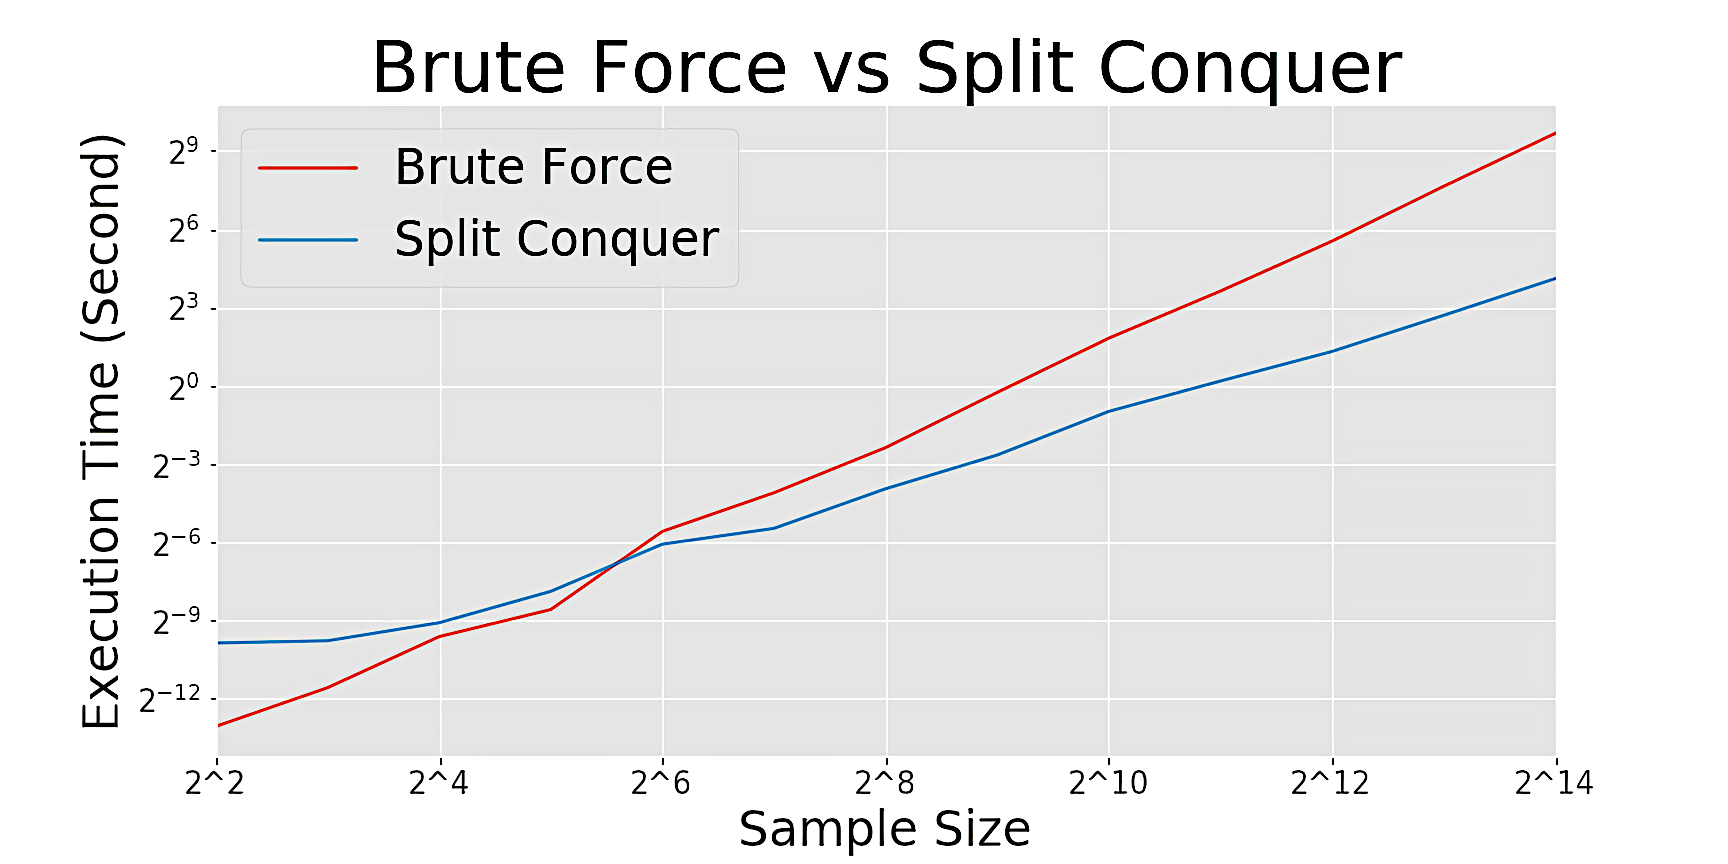
\includegraphics[scale=0.2]{comparison.jpg}
        \caption{Fonte: \href{https://towardsdatascience.com/basic-algorithms-finding-the-closest-pair-5fbef41e9d55}{Basic Algorithms — Finding the Closest Pair}}
    \end{figure}

\end{document}
